% THIS IS SIGPROC-SP.TEX - VERSION 3.1
% WORKS WITH V3.2SP OF ACM_PROC_ARTICLE-SP.CLS
% APRIL 2009
%
% It is an example file showing how to use the 'acm_proc_article-sp.cls' V3.2SP
% LaTeX2e document class file for Conference Proceedings submissions.
% ----------------------------------------------------------------------------------------------------------------
% This .tex file (and associated .cls V3.2SP) *DOES NOT* produce:
%       1) The Permission Statement
%       2) The Conference (location) Info information
%       3) The Copyright Line with ACM data
%       4) Page numbering
% ---------------------------------------------------------------------------------------------------------------
% It is an example which *does* use the .bib file (from which the .bbl file
% is produced).
% REMEMBER HOWEVER: After having produced the .bbl file,
% and prior to final submission,
% you need to 'insert'  your .bbl file into your source .tex file so as to provide
% ONE 'self-contained' source file.
%
% Questions regarding SIGS should be sent to
% Adrienne Griscti ---> griscti@acm.org
%
% Questions/suggestions regarding the guidelines, .tex and .cls files, etc. to
% Gerald Murray ---> murray@hq.acm.org
%
% For tracking purposes - this is V3.1SP - APRIL 2009

\documentclass{acm_proc_article-sp}
\usepackage{graphicx}
\graphicspath{ {Figures/} }
\usepackage[capposition=top]{floatrow}

\usepackage{lipsum}
\usepackage{multirow, tabularx, caption, booktabs}
\usepackage{makecell}
\renewcommand\cellalign{rc}
\usepackage{siunitx}
\sisetup{table-format=1.1}

\begin{document}

\title{What Works for Whom? }
\subtitle{A Bayesian Approach to Channeling Big Data Streams for Policy Analysis}
%
% You need the command \numberofauthors to handle the 'placement
% and alignment' of the authors beneath the title.
%
% For aesthetic reasons, we recommend 'three authors at a time'
% i.e. three 'name/affiliation blocks' be placed beneath the title.
%
% NOTE: You are NOT restricted in how many 'rows' of
% "name/affiliations" may appear. We just ask that you restrict
% the number of 'columns' to three.
%
% Because of the available 'opening page real-estate'
% we ask you to refrain from putting more than six authors
% (two rows with three columns) beneath the article title.
% More than six makes the first-page appear very cluttered indeed.
%
% Use the \alignauthor commands to handle the names
% and affiliations for an 'aesthetic maximum' of six authors.
% Add names, affiliations, addresses for
% the seventh etc. author(s) as the argument for the
% \additionalauthors command.
% These 'additional authors' will be output/set for you
% without further effort on your part as the last section in
% the body of your article BEFORE References or any Appendices.

\numberofauthors{3} %  in this sample file, there are a *total*
% of EIGHT authors. SIX appear on the 'first-page' (for formatting
% reasons) and the remaining two appear in the \additionalauthors section.
%
\author{
% You can go ahead and credit any number of authors here,
% e.g. one 'row of three' or two rows (consisting of one row of three
% and a second row of one, two or three).
%
% The command \alignauthor (no curly braces needed) should
% precede each author name, affiliation/snail-mail address and
% e-mail address. Additionally, tag each line of
% affiliation/address with \affaddr, and tag the
% e-mail address with \email.
%
% 1st. author
\alignauthor
Mariel Finucane\\
       \affaddr{Mathematica Policy Research}\\
       \affaddr{Cambridge, MA}\\
       \email{MFinucane@mathematica-mpr.com}
% 2nd. author
\alignauthor
Ignacio Martinez\\
       \affaddr{Mathematica Policy Research}\\
       \affaddr{Washington, DC}\\
       \email{IMartinez@mathematica-mpr.com}
% 3rd. author
\alignauthor Scott Cody\\
       \affaddr{Mathematica Policy Research}\\
       \affaddr{Cambridge, MA}\\
       \email{Scody@mathematica-mpr.com}
}
% There's nothing stopping you putting the seventh, eighth, etc.
% author on the opening page (as the 'third row') but we ask,
% for aesthetic reasons that you place these 'additional authors'
% in the \additional authors block, viz.
\date{31 July 2015}
% Just remember to make sure that the TOTAL number of authors
% is the number that will appear on the first page PLUS the
% number that will appear in the \additionalauthors section.

\maketitle
\begin{abstract}
In the coming years, public programs will continuously capture even more and richer data than they do now, including data from web-based tools used by participants in employment services, from tablet-based educational curricula, and from electronic health records for Medicaid beneficiaries, just for example.
Policy evaluations seeking to take full advantage of the volume and velocity of these data streams will require novel statistical methods. 
In this paper, we present just such a method, a Bayesian approach to randomized policy evaluations that efficiently estimates heterogeneous treatment effects, identifying what works for whom. 
The approach enables evaluators to consider multiple candidate interventions simultaneously, matching each study subject with the intervention that is most likely to benefit him or her. 
The trial design adapts to accumulating evidence: over the course of a trial, more study subjects are allocated to treatment arms that are more promising, given the specific subgroup from which each subject comes. 
Using a randomized experiment of students in an online course as a motivating example, we conduct a simulation study to identify the conditions under which our Bayesian adaptive design can produce better inference and ultimately smaller trials. 
In particular, we describe conditions under which there is more than a 90 percent chance that inference from the Bayesian adaptive design is superior to inference from a standard design, using less than one-third the sample size. 
Under the right circumstances, then, the Bayesian adaptive approach we propose can channel streams of big data to efficiently learn what works for whom.
\end{abstract}


%A category including the fourth, optional field follows...
\category{C.1.1}{Econometric and Statistical Methods and Methodology}{Bayesian Analysis}[General]
\category{C.1.3}{Econometric and Statistical Methods and Methodology}{Estimation}[General]
\category{C.1.5}{Econometric and Statistical Methods and Methodology}{Statistical Simulation}[General]
\category{C.3.1}{Multiple or Simultaneous Equation Models}{Multiple Variables}[Treatment Effect Models]
\category{C.4.4}{Econometric and Statistical Methods}{Special Topics}[Statistical Decision Theory]
\category{C.5.4}{Econometric Modeling}{Quantitative Policy Modeling}
\category{C.5.5}{Econometric Modeling}{- Data Sets}[Modeling and Analysis]
\category{C.6.3}{Mathematical Methods}{ Programming Models}[Mathematical and Simulation Modeling: Computational Techniques - Simulation Modeling]
\category{C.9.0}{Design of Experiments}{General}

\terms{Methods}

\keywords{Bayesian statistics, adaptive design, hierarchical models, heterogeneous treatment effects, randomized control trials, rapid-cycle evaluation, big data} % NOT required for Proceedings

\section{Introduction}
We are caught in a data deluge, with unprecedented volumes of information being collected every day to measure policy innovations, their implementation, and the resulting outcomes. 
These data have great potential not only to expand our knowledge of what policies work at the population level, but also for exploring the frontier of what works for whom, studying heterogeneous treatment effects across specific subgroups of the population.

Randomized controlled trials (RCTs) are the gold standard for determining what works, providing valid causal inference that nonrandomized designs can only approximate, at best. But standard RCTs can be time consuming and expensive \cite{luce2009rethinking}. 
Moreover, using RCTs to understand what works for different subgroups of program participants will increase both the time and budget required for a standard RCT. 

Bayesian approaches to RCTs can help leverage big data more efficiently. 
In this paper, we present a Bayesian approach to social policy RCTs that adapts to accumulating evidence: over the course of the trial, more study subjects are allocated to treatment arms that are more promising, given the specific subgroup that each subject comes from. 
This approach, which is based on the design of two recent clinical drug trials \cite{barker2009spy, kim2011battle}, provides valid estimates of heterogeneous causal effects sooner and with smaller sample sizes than would be required in a traditional RCT. 
To our knowledge, this strategy has not yet been applied to social policy research. 

The need to understand what works for whom is pressing. 
Consider the wide array of public programs currently evaluated through RCTs: employment services for the unemployed, education tools for struggling readers, and supportive services for adolescents on Medicaid, to name a few. With a precise understanding of what works for whom, each of these programs could be better targeted to specific subgroups. 
Which employment strategies are more effective for long-term unemployed individuals, and which are more effective for dislocated workers? 
Which reading interventions work best for dyslexic students, and which for students with attention-deficit/hyperactivity disorder? 
Which strategies reduce pregnancy risk for adolescent Medicaid beneficiaries for whom English is their first language, and which are effective for English-as-a-second-language speakers? 
In the coming years, all of these programs will capture more and richer data than they do now, including data from web-based tools used by participants in employment services, from tablet-based educational curricula, and from electronic health records for Medicaid beneficiaries. 
Under the right circumstances, the Bayesian adaptive approach we propose can channel these streams of data to determine what works for whom, doing so more efficiently than a non-Bayesian approach.

But we do not need to wait for the future to see big data. 
Online education generates massive amounts of data that can be harnessed to understand key effectiveness questions. 
In this paper, we use the online education context as an illustrative example to examine the benefits and limitations of Bayesian adaptive design compared to the standard approach of randomizing with equal probability to each treatment arm throughout a study. 
In particular, we simulate a series of experiments to answer the following research questions: 
\begin{enumerate}
  \item	Does the Bayesian adaptive design succeed in allocating its experimental subjects to more effective treatment arms?
  \item	Does the Bayesian adaptive design produce better final inference?
  \item	Can the Bayesian adaptive design learn earlier and with smaller sample sizes what works for whom?
\end{enumerate}

Throughout, we focus on identifying the conditions under which the Bayesian adaptive design outperforms conventional methods according to each of these three criteria.

We first describe a particular online education experiment that motivates the analyses presented in this paper. 
We then detail the specific adaptive randomization algorithm that we propose. We present the methods and results of a simulation study that compares Bayesian adaptive versus standard randomized design. 
We then briefly describe two possible extensions of the method and conclude with a discussion of the limitations of the proposed approach.


\section{Data and Methods}
Martinez (2015) \cite{martinez2014never} conducted a nonadaptive randomized trial of students in a massive open online course to test whether changes in the way programs communicate with students can improve course completion rates. 
The RCT generated vast amounts of data on more than 23,000 course participants from 169 countries.  
In the final week of the course, students in the intervention arm received an email 'nudge' describing the negative correlation between procrastination and achievement. 
These students were 17 percent more likely to complete the course successfully the following week than students in the control group (p < 0.01). 
Additionally, in a post-hoc analysis, Martinez found that the treatment effect was heterogeneous across countries. 
For example, Germans assigned to the intervention arm were 167 percent more likely to complete the course (p = 0.04), but no effect was found for students from the United States (p = 0.94). 
Inspired by the rich data collected in this study and the evidence of heterogeneous effects, the current paper presents a simulation study investigating the potential advantages of conducting this experiment using a Bayesian adaptive design.

To allow analysis of what works for whom, we begin by envisioning a multiarm version of this two-arm trial. 
We ask, for example: Had the original design included additional treatment arms, would it have identified an effective intervention for students from the United States or from other countries that did not benefit from the intervention implemented in Martinez's study? 
In particular, we consider four nudging strategies at once and one control arm, and over the course of the (simulated) experiment attempt to match nudging strategies with the countries whose students are most likely to respond to them.

We consider a six-week course in which 26 cohorts of students participated over the course of a year, with start dates spaced two weeks apart. 
In the fifth week of each cohort, students who have been randomized to an intervention receive a 'nudge,' encouraging them to finish all assignments. 
The outcome of interest is successful completion of the course in week 6. 
As shown in Figure~\ref{fig:timeline}, this schedule assumes that outcomes from any given cohort are observed in time to inform randomization of the next cohort. 
We discuss two ways to loosen this assumption in the Discussion. 

\begin{figure}
\centering
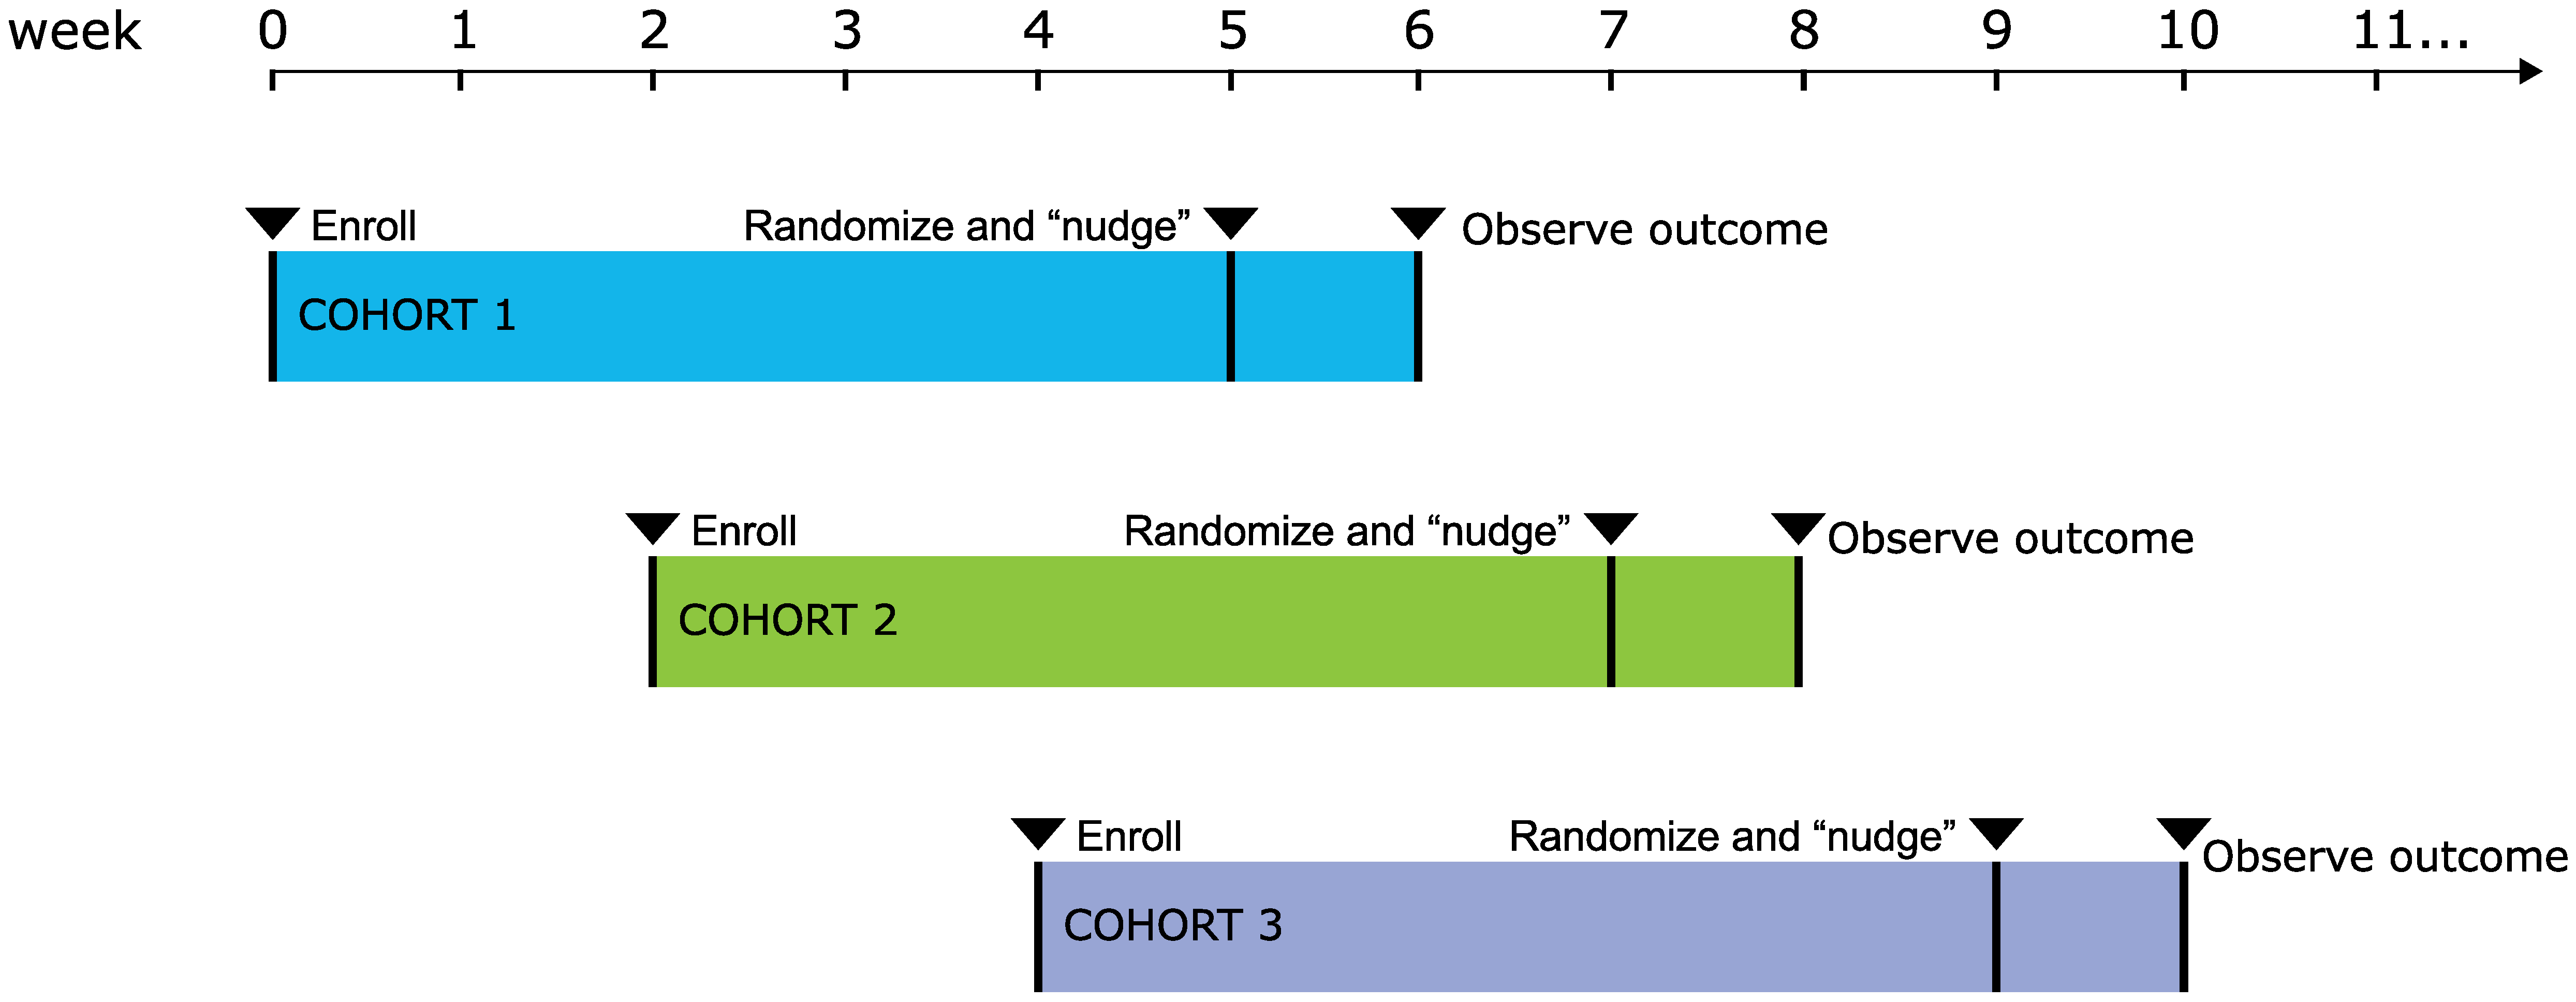
\epsfig{file=./Figures/Timeline.eps, width=\textwidth}
\caption{We consider a six-week course in which 26 cohorts of students participated over the course of a year, with start dates spaced two weeks apart. For illustrative purposes, we show the first 3 of 26 cohorts here.}
\label{fig:timeline}
\end{figure}

To answer our research questions, we compare two possible five-arm designs via simulation. 
The specific approach we use to simulate synthetic data sets under each of these designs is described in the next section. 
The remainder of this section describes the two designs: (1) a standard five-arm randomized design that uses equal randomization probabilities of 20 percent per arm throughout the study, and (2) a Bayesian adaptive design in which information gleaned in the earlier stages of the trial influences which nudging strategies are used in each country later in the trial such that---as the study progresses and we learn what works for whom---each subject has an increasing probability of being randomized to the treatment arm that is most effective in his or her country. 
By concentrating the sample size in those country-by-strategy pairs that seem most promising, we aim to increase our power to identify the most effective strategy in each country. 
Under the Bayesian adaptive design, starting with cohort 1, we thus pursue the goal of learning which nudging strategy is most effective for students from each country, as shown in Figure~\ref{fig:timeline2}. 

\begin{figure}
\centering
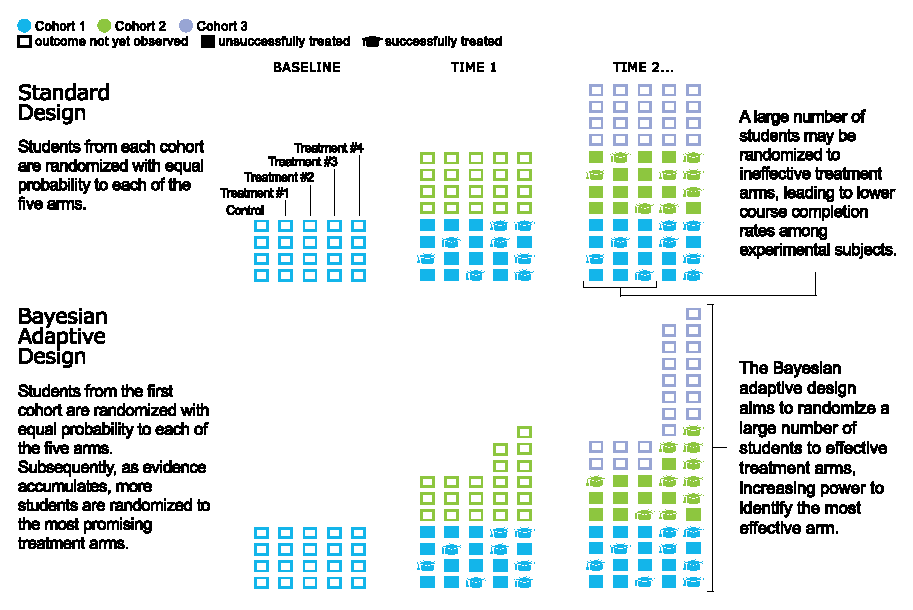
\epsfig{file=./Figures/vertchart.eps, width=\textwidth}
\caption{In each country, as evidence accumulates during the course of a Bayesian adaptive trial, more students are randomized to the treatment arms that are most promising.}
\label{fig:timeline2}
{\floatfoot{Note: At baseline (corresponding to weeks 0-5 in Figure~\ref{fig:timeline}), students from cohort 1 enroll and we randomize them to one of five treatment arms and nudge accordingly. At time 1, (corresponding to weeks 6 and 7 in Figure~\ref{fig:timeline}), we observe the course completion outcomes of students from cohort 1 and we randomize and nudge students from cohort 2. At time 2, (corresponding to weeks 8 and 9 in Figure~\ref{fig:timeline}), we observe the course completion outcomes of students from cohort 2 and we randomize and nudge students from cohort 3.}}
\end{figure}

We learn as we go, adapting our randomization scheme as follows:
\begin{itemize}
    \item Before the course begins, what works for whom is not known, so randomize cohort 1 with 20 percent probability to each of the five arms, and nudge accordingly.
    \item Observe who from cohort 1 completes the course.
    \item Use these data to update our understanding of which intervention arm is most effective for students in each country, by fitting a Bayesian model to the data from cohort 1. The model is described in the Appendix.
    \item For cohort 2, randomize students according to this updated understanding, with students randomized preferentially to the treatment arms that---based on the accumulated data---are estimated to be most effective in their country.
    \item Observe who from cohort 2 completes the course.
    \item Use these data to update our understanding again, by refitting the model to the data set that now includes students from cohorts 1 and 2.
    \item Randomize cohort 3 accordingly.
    \item Observe who from cohort 3 completes the course.
    \item Continue to adapt the randomization scheme in this fashion for cohorts 4 through 26.
\end{itemize}

Although some current approaches to policy evaluation are adaptive in limited ways (for example, those with early stopping rules if an intervention is wildly successful or clearly harmful), the standard, frequentist statistical paradigm inhibits flexible adaptation with its requirement that all possible study outcomes be prespecified. Under the Bayesian paradigm, by contrast, researchers are only required to prespecify---using formal, probabilistic statements of uncertainty---how a design will change as evidence accumulates \cite{berry2006bayesian, george1994stopping}. In this way, the Bayesian approach learns continually from every cohort's outcomes rather than incorporating new information only at widely spaced intervals. We will show that this flexibility facilitates efficient determination of what works for whom by making optimal use of data as they are collected.

We pair this Bayesian adaptive design with a hierarchical Bayesian approach to analysis. This approach enables us to ‘borrow strength' across countries, refining our understanding of an intervention's effectiveness for each specific country by drawing on data from other countries in the region, to the extent that the data support such a linkage. For example, in inferring whether a given nudging strategy is effective in India, we take a weighted average of the proportion of Indian course completers who received the nudge with the proportion of South Asian course completers who received the nudge. The weights are not specified in advance, but rather determined by (1) the degree of concordance across results from different countries within a region and (2) the strength of the evidence based on data for Indian students alone. More weight will be assigned to the contextual region-level (i.e., South Asian) data in those cases with a high degree of concordance or when the country-specific (i.e., Indian) evidence is weak, for example due to a small sample size in India. Similarly, inference for any specific region draws on data from the other regions of the world. For example, because the course Martinez studied included only eight students from the region of Oceania, the Bayesian hierarchical model borrows strength from other regions to make estimates in those small island nations. Borrowing strength across countries within a region and across regions of the globe---to the extent determined by the data---can produce more precise, more predictive inference \cite{gelman2014bayesian} and ultimately smaller, less costly trials \cite{berry2010bayesian}.

\section{Simulation Study}
To compare the Bayesian adaptive design's performance to that of the standard method of subject allocation in randomized trials, we simulate and analyze synthetic data sets. To identify the conditions under which the Bayesian adaptive design produces benefits, we simulate data sets under each of nine scenarios characterized by different sample sizes and different effect sizes. However, acknowledging that in any given simulated data set the Bayesian adaptive design might perform better or worse than the standard design just by chance alone, we conduct 1,000 simulations of each of the two designs in each of the nine scenarios. In each scenario, we thus simulate and analyze 1,000 synthetic data sets using the standard approach and 1,000 synthetic data sets using the proposed approach.

For each simulation, we assume a true course completion rate in each country under each of the five treatment arms. For example, in the control arm in the United States, the first simulation might assume that the true course completion rate is 4 percent. We then generate two synthetic data sets, one under the Bayesian adaptive design and one under the standard design. In each case, we randomly assign computer-generated 'students' to each of the five treatment arms, with randomization probabilities chosen for each design as we describe in the Methods section. We randomly generate simulated course completion outcomes for each synthetic student in each data set, with probability corresponding to the assumed truth, given the student's country and assigned treatment arm. For example, if the first synthetic student from the first simulation was from the United States and was randomized to the control arm, with 4 percent probability we would say that the student had completed the course and with 96 percent probability we would say that the student had not completed the course. For simplicity, the simulation design assumes that each cohort comprises 1/26 of the total sample size.

In choosing the true course completion rates, we assume that---on average across countries---two of the intervention arms are effective and two are no more effective than control. As we will show in the Results section, the difference in the probability of course completion of students assigned to effective versus ineffective arms is an important determinant of the performance of the Bayesian design. We therefore consider three values of this difference. In addition to these mean effect sizes, we assume regional and country-level heterogeneity, to allow some interventions to be more or less effective in some regions or countries than others, with the magnitude of heterogeneity chosen to reflect the true amount of heterogeneity that Martinez observed. The Appendix details the process through which we induce this heterogeneity. We also consider three possible sample sizes. The pair-wise combinations of mean effect size and total sample size characterize the nine scenarios we consider to assess the conditions under which our Bayesian approach performs more and less well. The values of each factor that we consider are:
\begin{itemize}
    \item Mean effect size (i.e., the difference in the probability of course completion of students assigned to effective versus ineffective arms), averaging across countries: small, medium, and large, as detailed in the Table. 
    \item Sample size: 10, 50, and 100 percent of the actual sample size of 23,461 students.
\end{itemize}

\begin{table}
    \linespread{0.9}
\centering
\caption{Three possible values of the difference in the probability of course completion of students assigned to effective versus ineffective treatment arms.}
\label{my-label}
\begin{tabular}{rSSS}
\thead{Mean effect size,\\
       averaging across \\countries} 
    &   \multicolumn{2}{c}{\thead{Probability of \\ 
                                  course completion (\%)}}
            &   {\thead{Difference}}                           \\
    &   {\thead{Ineffective\\ arms}}
        &   {\thead{Effective\\ arms}} 
            &                                                   \\
    \hline
Small   & 4.6   & 5.3   & 0.8 \\
Medium  & 4.6   & 8.5   & 3.9 \\
Large   & 4.6   & 13.3  & 8.7
\end{tabular}
\begin{flushleft}
{\footnotesize{Note: The probabilities of course completion given a small mean effect size are equal to those observed by Martinez. For the medium and large mean effect sizes, the difference values were chosen to be 0.5 and 1 units greater on the logit scale than the treatment-control difference observed by Martinez. Throughout, we assume that---on average across countries---two of the intervention arms are effective and two are no more effective than the control.}}
\end{flushleft} 
\end{table}

\section{Results}
In this section we show that Bayesian adaptive design offers a promising new approach for improving policy evaluation. 
In particular, we demonstrate advantages against the standard approach in terms of (1) the successful allocation of experimental subjects to more effective treatment arms, (2) the final inference produced, and (3) the total sample size required. 

\subsection{Does the Bayesian adaptive design succeed in allocating its experimental subjects to more effective treatment arms?}
The Bayesian adaptive design takes advantage of the information learned during the course of the experiment, successfully assigning more students to more effective treatment arms during the trial. Figure~\ref{fig:3} shows that, as a result, it nudges more of its experimental subjects to complete the course than does the standard design. This is the case in at least 50 percent of simulations for all nine combinations of sample size and mean effect size that we consider, as shown in the figure using horizontal black lines in the middle of each box plot. For five of the nine combinations (when the mean effect size is large, and---for the full sample size and for 50 percent of the full sample size---when the effect size is medium), this is the case in all 1,000 simulations. In these five scenarios, we observe median increases of at least 30 percent in course completion rates among experimental subjects. 

\begin{figure}
\centering
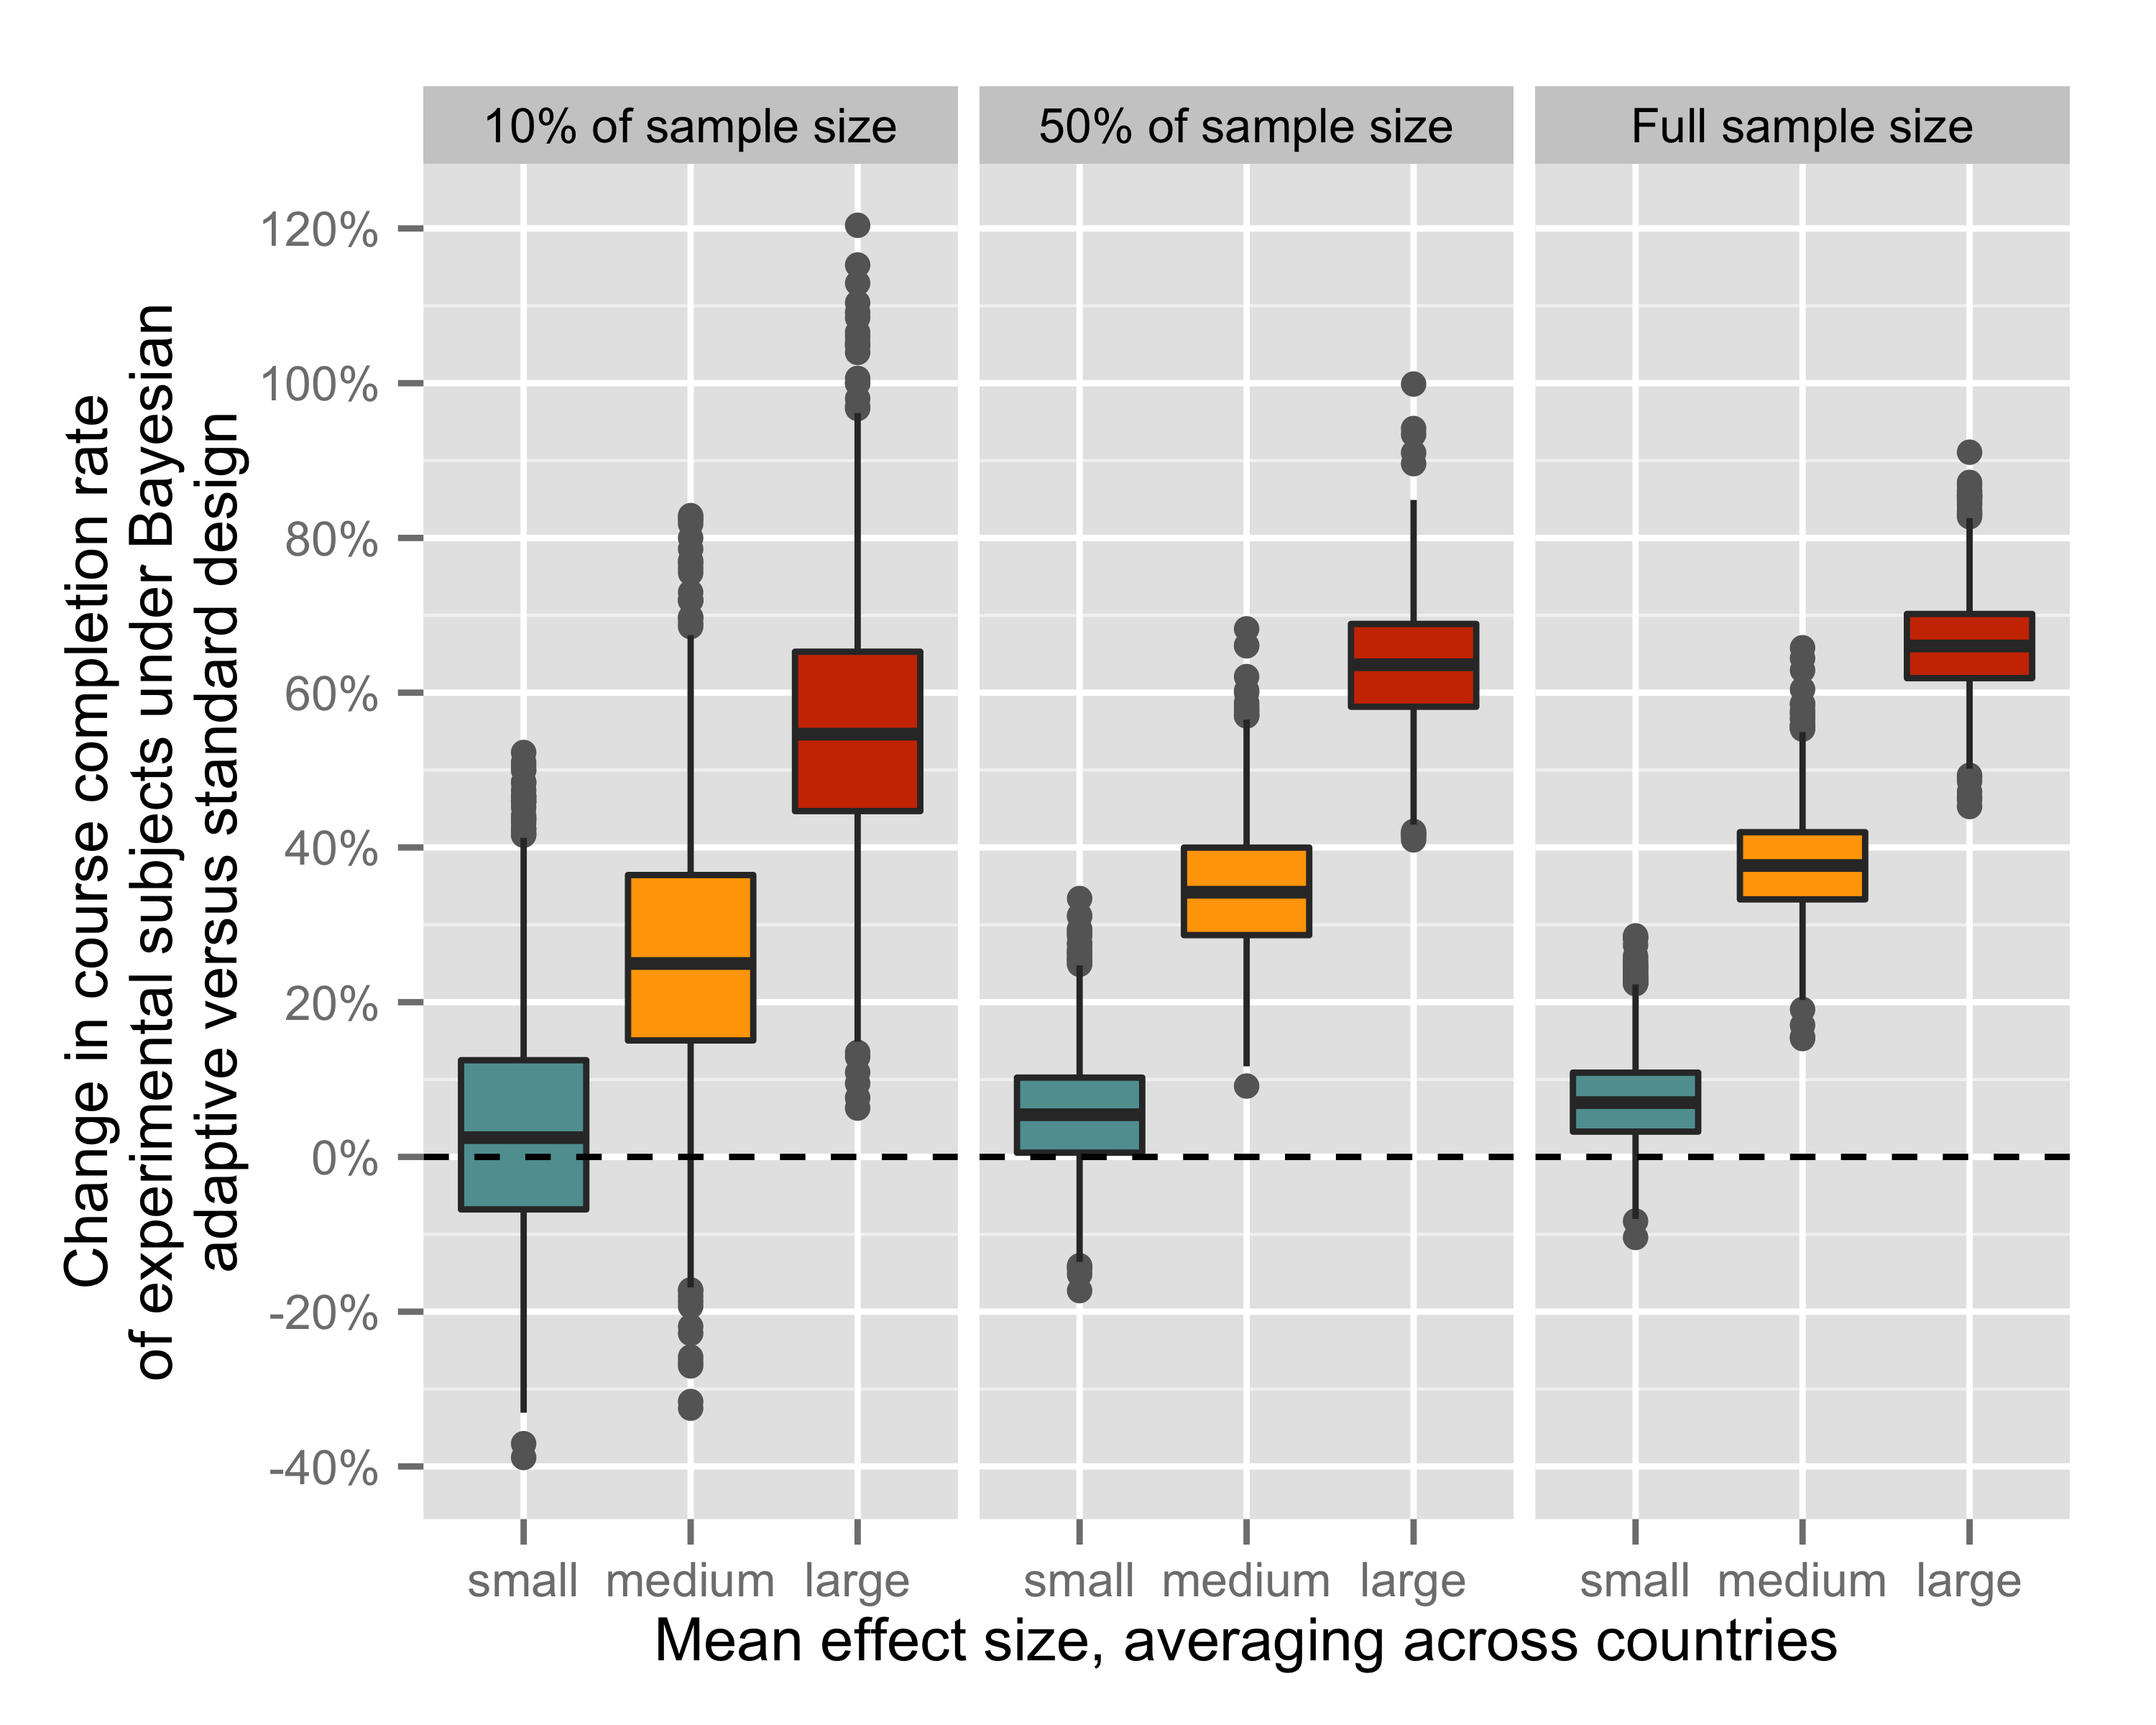
\includegraphics[width=\textwidth]{fig3}
\caption{The Bayesian adaptive design successfully allocates its experimental subjects to more effective treatment arms than the standard design.}
\label{fig:3}
{\floatfoot{Note: For each of the nine scenarios considered, a boxplot summarizes the distribution across 1,000 simulations of the percent change in the course completion rate of experimental subjects of the Bayesian adaptive design compared to the standard design. For example, a y-axis value of 20 percent indicates a simulation in which the course completion rate of experimental subjects is 20 percent higher under the Bayesian adaptive design than under the standard design. In each boxplot, the horizontal black line depicts the median of the distribution; the upper and lower ``hinges'' depict the 25th and 75th percentiles; the ``whiskers'' extend from the hinges to the most extreme values that are within 1.5 times the inter-quartile range; outliers beyond the end of the whiskers are plotted as points.}}
\end{figure}

Across sample sizes, we note that the Bayesian adaptive design is especially successful at increasing the course completion rate of its experimental subject when the mean effect size is large. This is because when effect sizes are larger, the effective treatment arms to which the Bayesian design succeeds in allocating its subjects are associated with higher probabilities of course completion. 

\subsection{Does the Bayesian adaptive design produce better final inference?}
We next turn to the important question of whether the Bayesian adaptive design produces better final inference than the standard design. We quantify the quality of the final inference using the following measure of predictive performance: Based on the final inference from the Bayesian adaptive design, choose a ``best'' nudging strategy in each country. Now enroll a new cohort of students in the next edition of the course. Nudge each student using the chosen strategy for his or her country. How many more students from this new cohort would be expected to complete the course using this strategy than had their nudge been chosen based on inference from the standard design? 
As shown in Figure 4, the Bayesian adaptive design outperforms the standard design by this metric in at least 50 percent of simulations for all nine combinations of sample size and mean effect size that we consider. It performs better in at least 95 percent of simulations in four of the nine scenarios (for the full sample size and for 50 percent of the full sample size, when the mean effect size is medium or large). These gains are achieved because the Bayesian adaptive design---by concentrating sample size in those treatment arms that seem most promising---achieves more power to compare successful treatments that differ in effectiveness only slightly. This higher power enables the Bayesian adaptive design to distinguish among successful treatment arms, ultimately identifying the most effective. 

\begin{figure}
\centering
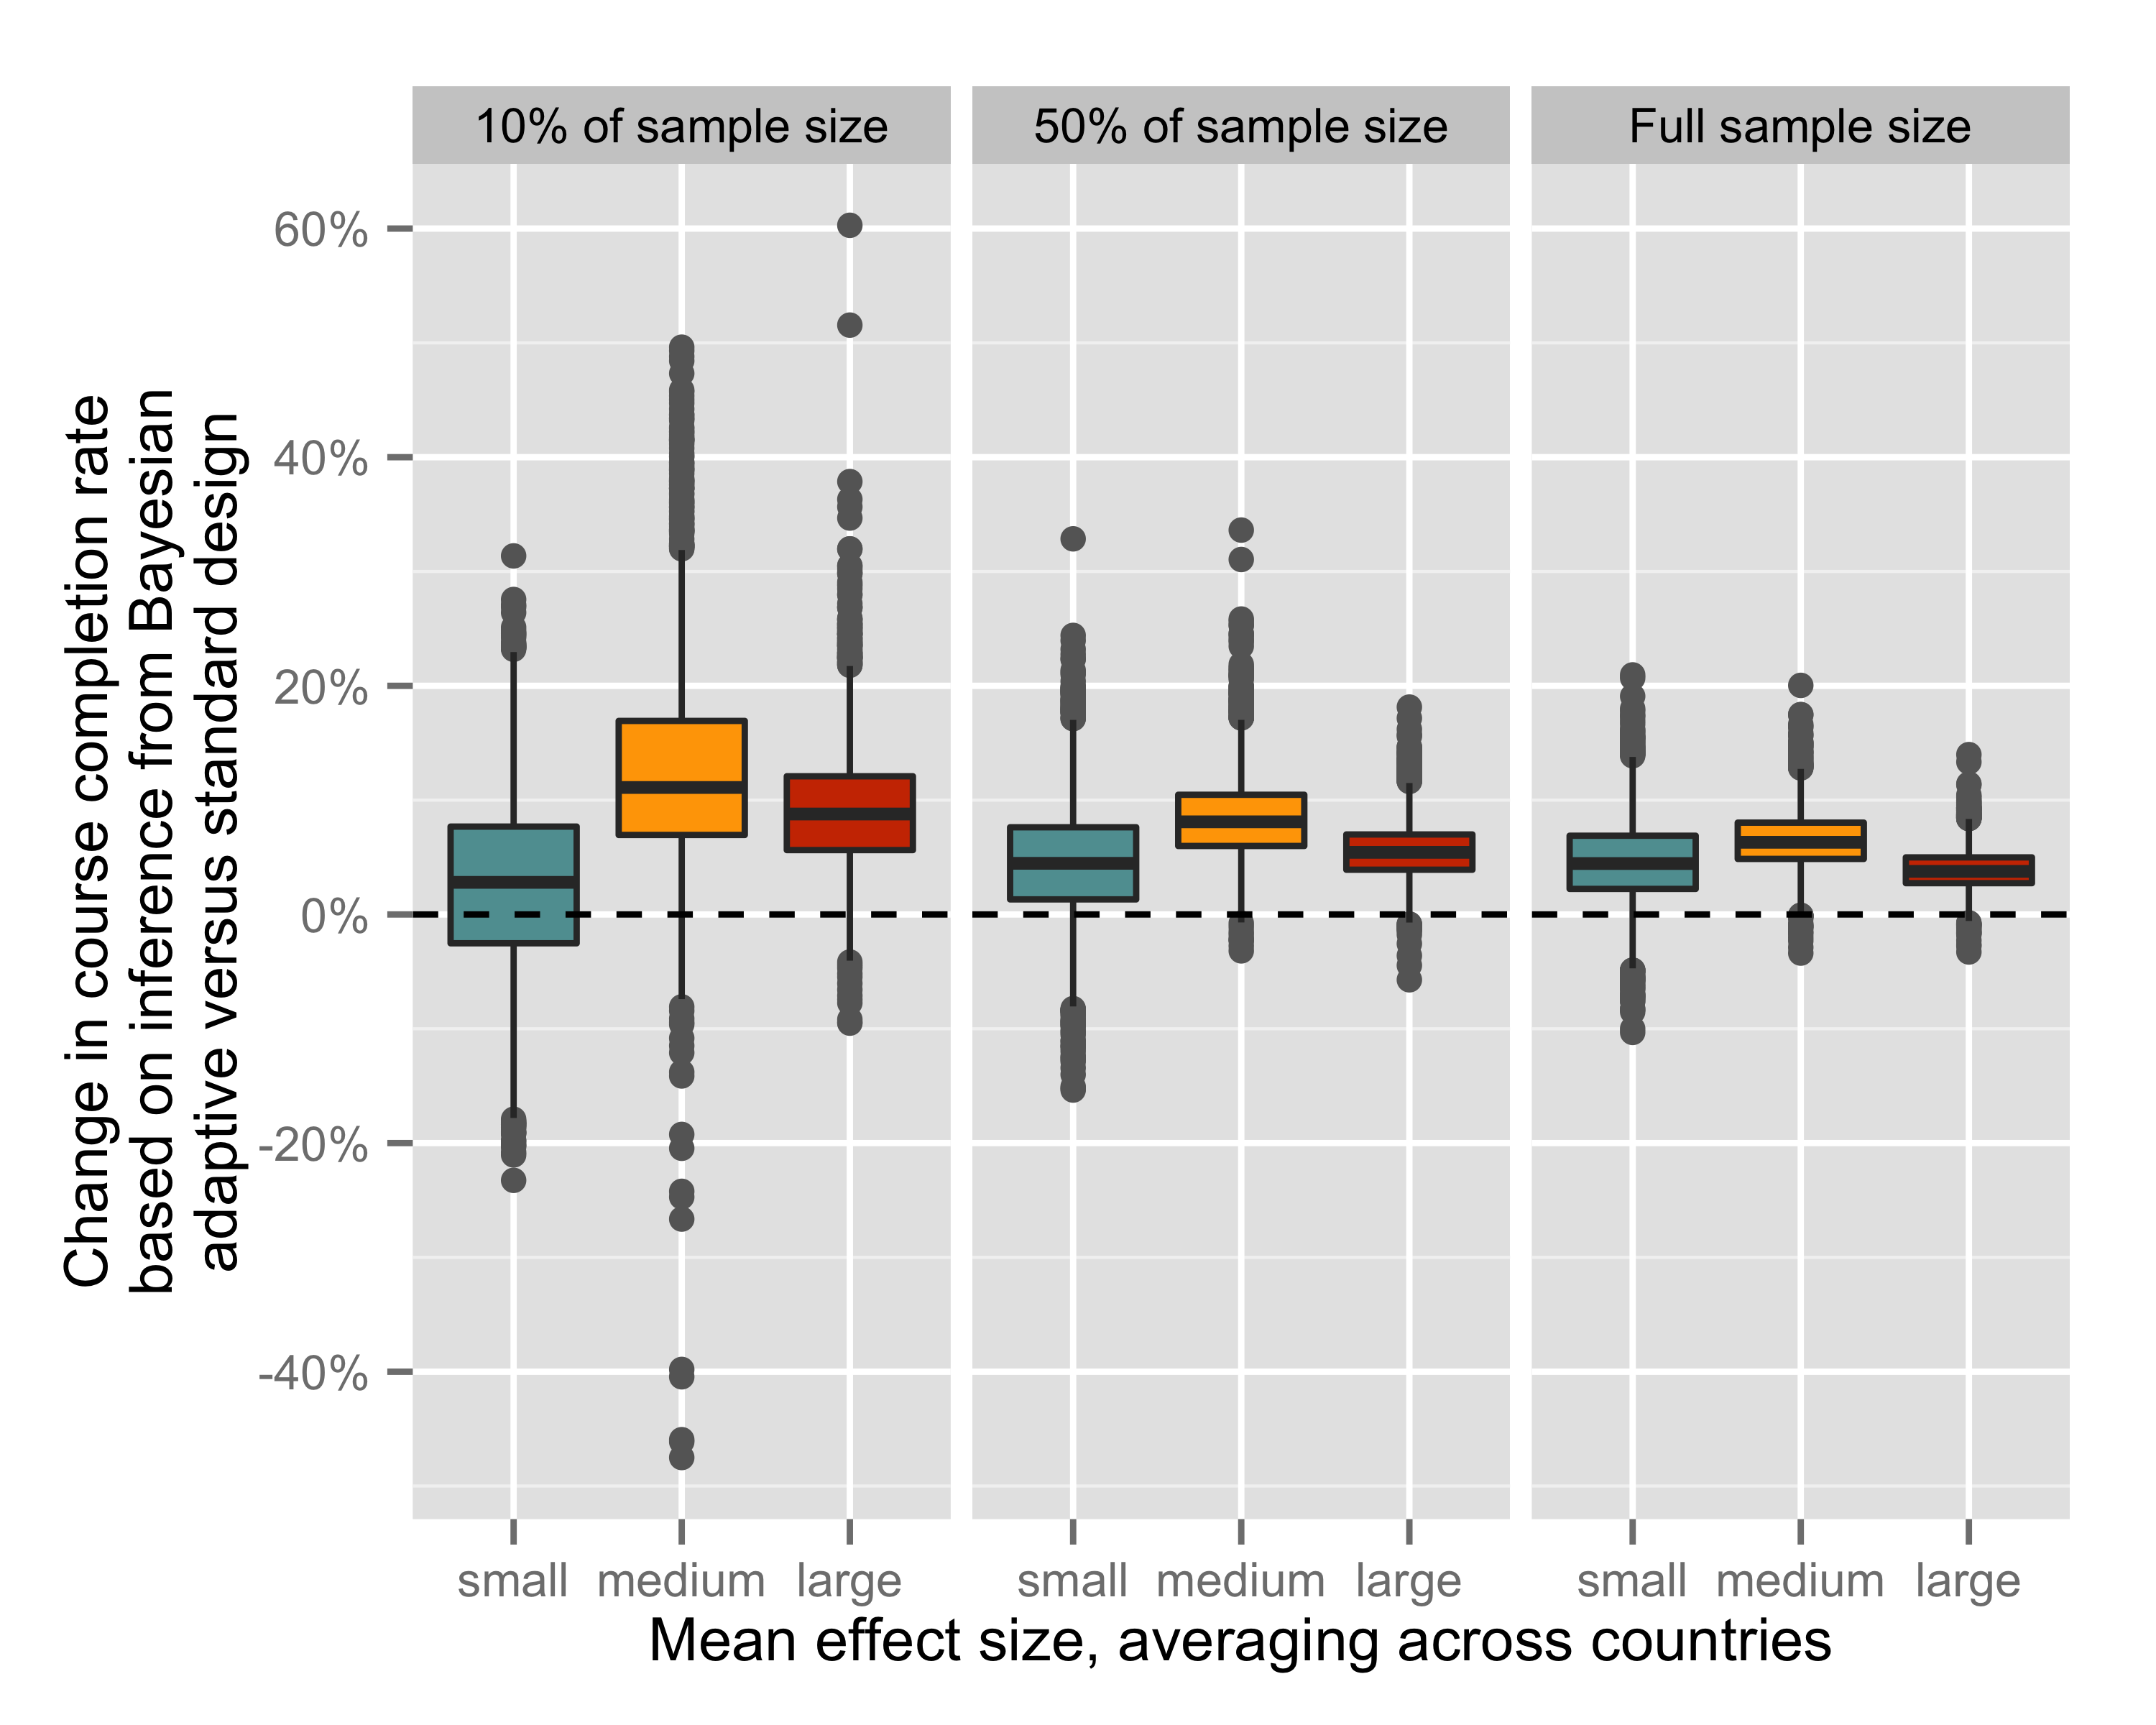
\includegraphics[width=\textwidth]{fig4}
\caption{The Bayesian adaptive design produces better final inference than the standard design.}
\label{fig:4}
{\floatfoot{Note: For each of the nine scenarios considered, a boxplot summarizes the distribution across 1,000 simulations of the percent change in the course completion rate based on inference from the Bayesian adaptive design compared to inference from the standard design. For example, a y-axis value of 20 percent indicates a simulation in which the course completion rate increases by 20 percent if you choose which arm to assign students to based on the results of the Bayesian adaptive design versus if you choose based on the results of the standard design. In each boxplot, the horizontal black line depicts the median of the distribution; the upper and lower ``hinges'' depict the 25th and 75th percentiles; the ``whiskers'' extend from the hinges to the most extreme values that are within 1.5 times the inter-quartile range; outliers beyond the end of the whiskers are plotted as points.}}
\end{figure}

Whereas Figure~\ref{fig:4} showed large benefits of the Bayesian adaptive design for large effect sizes, this metric shows the biggest gains for medium effect sizes. This is because, given large effect sizes, the standard design can often successfully identify the best treatment arm, leaving less room for improvement. 
We now consider which types of countries benefit most from the Bayesian adaptive design, in terms of the final inference produced. We consider only a single combination of sample size and mean effect size: the full sample size with small mean effect sizes, corresponding to the actual conditions of Martinez's study. Figure~\ref{fig:5} shows that the Bayesian adaptive design produces better inference in all countries, that the benefits are largest in countries with around 100 students, and that there are diminishing returns in very large countries, where large sample sizes enable the standard design to successfully identify the best treatment arm. 

\begin{figure}
\centering
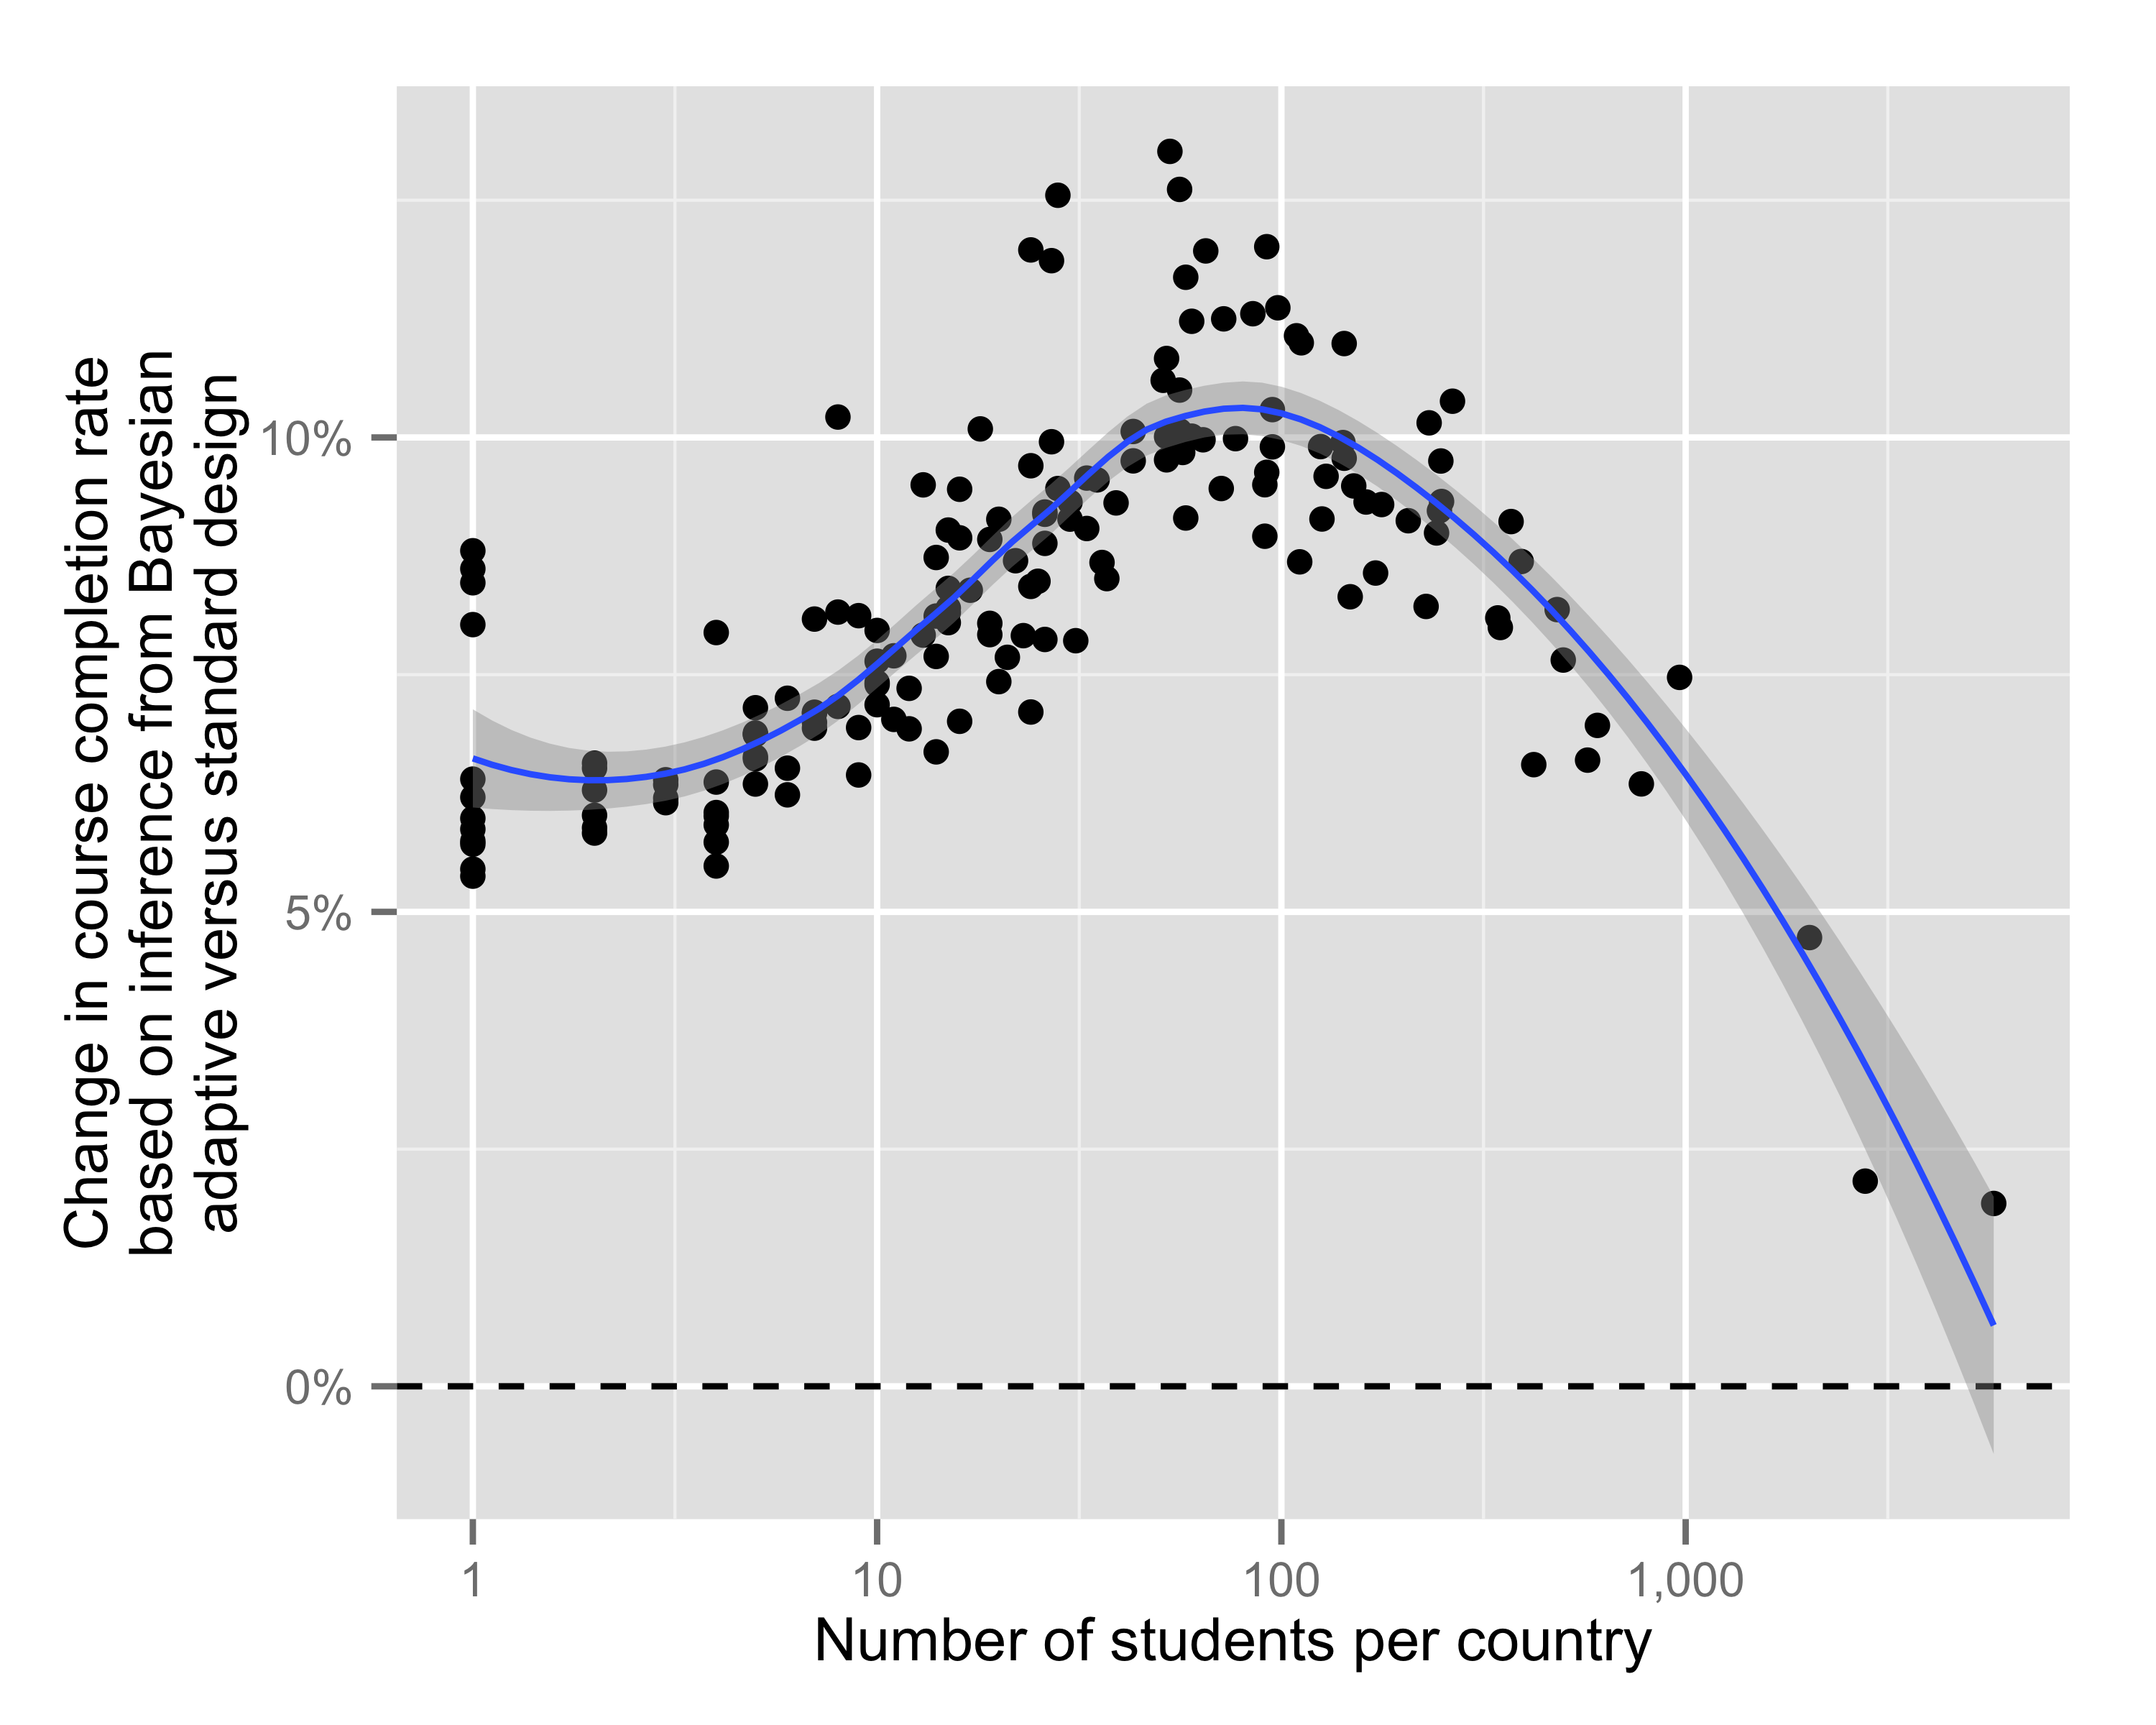
\includegraphics[width=\textwidth]{fig5}
\caption{The Bayesian adaptive design produces better inference than the standard design in all countries, and the benefits are largest in medium-sized countries.}
\label{fig:5}
{\floatfoot{Note: Averaging across the 1,000 simulations, we show the percent change in each country of the course completion rate based on inference from the Bayesian adaptive design compared to inference from the standard design. For example, a y-axis value of 20 percent indicates a country in which the course completion rate increases by an average of 20 percent if you choose which arm to assign students to based on the results of the Bayesian adaptive design versus if you choose based on the results of the standard design. The x-axis shows the country’s sample size. We consider only a single combination of sample size and mean effect size (the full sample size with small mean effect sizes, corresponding to the actual conditions of Martinez’s study). The blue line shows a loess smooth, and the grey shading shows a 95 percent confidence interval around the smooth.}}
\end{figure}

\subsection{Can the Bayesian adaptive design learn earlier and with smaller sample size what works for whom?}
Our final analysis determines how early in the study the Bayesian adaptive design learns what works for whom. In particular, using the same metric of predictive performance, we compare inference produced by the Bayesian adaptive design after each cohort of students is enrolled to the inference produced by the standard design after the full experiment. Figure~\ref{fig:6} indicates a high probability that inference from the Bayesian adaptive design after enrolling only a small number of cohorts is superior to the inference that the standard design achieves after the full experiment. In particular, in all nine scenarios, there is at least a 50 percent chance that inference from the Bayesian adaptive design after enrolling only 6 cohorts already surpasses inference produced by the standard design after enrolling all 26 cohorts. For the full sample size and for 50 percent of the full sample size, when the mean effect size is medium or large, there is more than a 90 percent chance that inference from the Bayesian adaptive design after enrolling only 7 cohorts surpasses inference produced by the standard design after enrolling all 26 cohorts. 

\begin{figure}
\centering
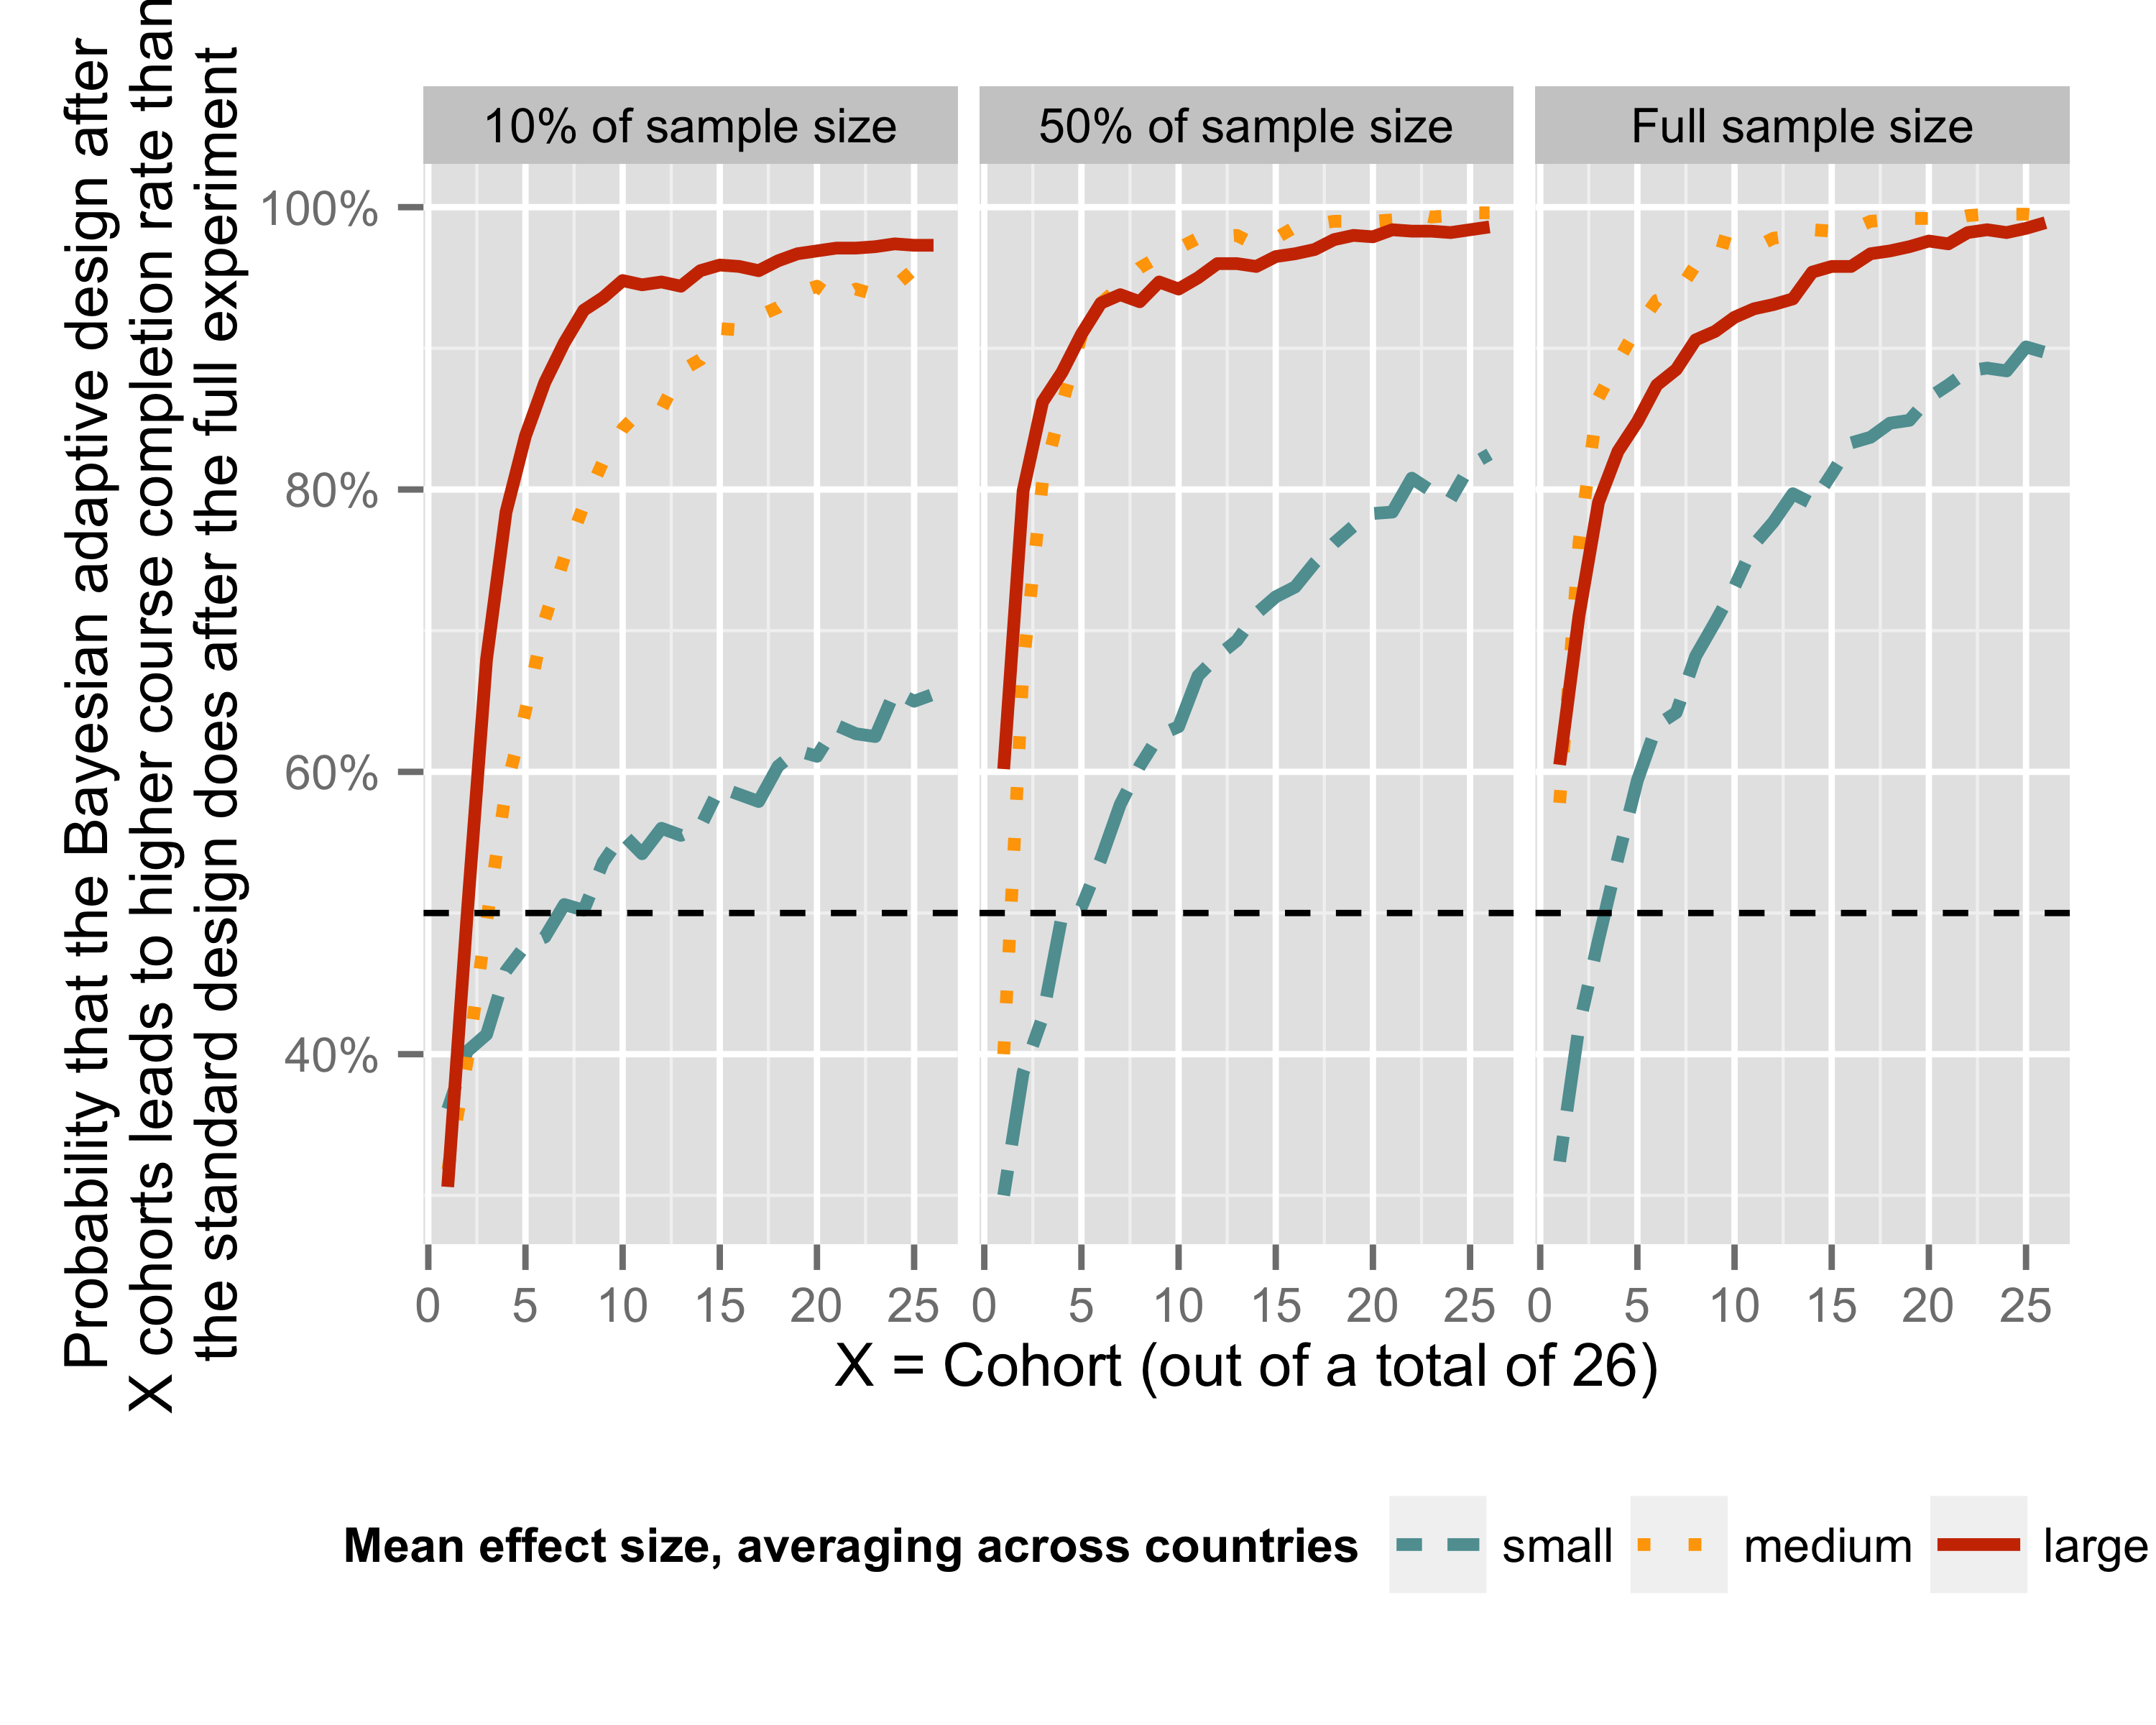
\includegraphics[width=\textwidth]{fig6}
\caption{The Bayesian adaptive design learns what works for whom earlier in the study than the standard design}
\label{fig:6}
{\floatfoot{Note: We compare the two designs using the following measure of predictive performance. Based on the inference from the Bayesian adaptive design after collecting X cohorts worth of data, choose a ``best'' nudging strategy in each country. Now enroll a new cohort of students in the next edition of the course. Nudge each student using the chosen strategy for his or her country. Would more students be expected to complete the course using this strategy than had their nudge been chosen based on inference from the standard design after collecting all 26 cohorts' worth of data? After each cohort, in each simulation, we determine whether the Bayesian adaptive design would produce better inference by this metric. We calculate the probabilities shown here as the proportion of simulations for which this is the case. For example, for an x-axis value of 10 cohorts, a y-axis value of 60 percent indicates that in 60 percent of simulations, course completion rates based on analyzing 10 cohorts' worth of data from the Bayesian adaptive design were higher than those based on an analysis of all 26 cohorts' worth of data from the standard design.}}
\end{figure}

\section{Extensions}
In this section, we briefly present two possible extensions to this design. First, we consider the case in which not all treatment arms are equally costly. A feature of the Bayesian paradigm is that is ideally suited for formal decision analysis that explicitly considers the costs of different approaches. For example, rather than adapting randomization based on the probability that a given treatment arm is the most effective in a given country, we could instead adapt based on the probability that each of three candidate treatment arms was at least X times as effective as the control, while adapting randomization to a fourth expensive candidate treatment arm based on the probability that it outperformed the next best option by at least Y fold, with X and Y reflecting the relative monetary and nonmonetary costs of each intervention.
Second, we consider extending the proposed method to rapid-cycle evaluation (RCE), which tests whether changes to a program's operations result in better outcomes. Program administrators can use RCE to test changes in when, where, or how they provide services; changes to their administrative procedures; and even changes to how they communicate with program participants. In many situations, program administrators want to know which operational approaches work best for which types of participants. The goal is often not to provide a one-time, summative assessment of an entire program but rather to provide ongoing decision support to program administrators for continual quality improvement.
Adaptive design is uniquely well suited to RCE. The Bayesian adaptive framework could be incorporated into RCEs to test multiple changes with the goal of identifying heterogeneous treatment effects. To determine when sufficient evidence has amassed that a given intervention is effective, rigorous decision rules could be incorporated into the Bayesian adaptive design described in this paper; at this point, the intervention would graduate from the evaluation and be incorporated into daily program operations. Conversely, if sufficient evidence amasses that a given intervention is ineffective, that arm could be closed. As effective approaches graduate and ineffective approaches are dropped from the RCE, this would make room for newly available interventions, without having to restart the evaluation. In this way, Bayesian adaptive design would allow RCE experiments to be integrated into the ongoing flow of program operations. By building such a platform for continuous improvement into program operations, administrators could be sure that they were always comparing the alternatives most relevant to current decision-making.

\section{Discussion}
Although Bayesian adaptive design can be applied to a variety of programs, the programs must have two things in common: (1) rolling enrollment and (2) outcomes that can be observed soon enough to permit adaptation of the trial design. Regarding the second requirement, recall that the simulation study presented here assumes that we are able to observe the outcome of interest for all students in a given cohort before randomizing students from the next cohort. However, we note that the method is generalizable to instances when this is not the case. If more time were needed between the intervention and measurement of the outcome, we could structure things differently. For example, outcomes from cohort 1 could inform randomization of cohort 5; outcomes from cohorts 1 and 2 could inform randomization of cohort 6; and so on. Alternatively, unobserved final outcomes could be imputed based on intermediate outcomes to permit adaptation of the trial design before final outcomes become observable.
In addition to these two restrictions, another important challenge of applying the proposed methodology is an operational one. The program under investigation must be able to pivot quickly, continuously accommodating new data as they become available. 
The example presented here examines heterogeneous effects by subgroups, but Bayesian adaptive design could also be used to determine the relative effectiveness of treatments population-wide. However, to the extent that subgroups are of interest, they present additional methodological requirements. In particular, the subgroups must be observable at baseline, and they must explain at least a portion of the heterogeneity of effects.
To successfully carry out Bayesian adaptive design, researchers will require access to powerful computational resources. Because simple sample size formulas for complex Bayesian hierarchical models do not exist, the properties of a given design are assessed via simulation, as we have done here. Even for 'small data' trials, Bayesians must thus perform 'big data' simulations at the design phase. Furthermore, Bayesian software is not as refined as frequentist software (e.g., SAS, Stata). It is therefore often the case that Bayesian statisticians must code their own computational routines by hand, which is time consuming and requires validation. Lastly, many Bayesian models are fit using iterative algorithms that often require longer computer run times than their frequentist counterparts. These three factors combine to create a substantial computational burden. For example, the results presented in this paper required more than 1,000 core-hours on Amazon's Web Services platform. 
Bayesian statistical computing is a very active area of research, however, with revolutionary new computational techniques developed just in the past decade. Such techniques, coupled with important advances in high-speed computing, have made the current study computationally feasible. We foresee and look forward to a time in the near future when further progress renders computational constraints even less salient.

\section{Conclusion}
In this era of big data, the demand for policy evaluations that are simultaneously cheaper and more informative is increasing. In particular, there is demand for researchers to take full advantage of the volume and velocity of data that are now routinely collected during policy research, to efficiently answer the important question of what works for whom. A danger is that this demand might tempt researchers to abandon the rigorous methods such as RCTs that are crucial for making valid causal inference about program impacts. In this paper, we presented a novel Bayesian approach that produces better inference more efficiently than the standard approach, without sacrificing crucial methodological principles.

%ACKNOWLEDGMENTS are optional
\section{Acknowledgments}
This section is optional; it is a location for you
to acknowledge grants, funding, editing assistance and
what have you.  In the present case, for example, the
authors would like to thank Gerald Murray of ACM for
his help in codifying this \textit{Author's Guide}
and the \textbf{.cls} and \textbf{.tex} files that it describes.

%
% The following two commands are all you need in the
% initial runs of your .tex file to
% produce the bibliography for the citations in your paper.
\bibliographystyle{abbrv}
\bibliography{sigproc}  % sigproc.bib is the name of the Bibliography in this case
% You must have a proper ".bib" file
%  and remember to run:
% latex bibtex latex latex
% to resolve all references
%
% ACM needs 'a single self-contained file'!
%
%APPENDICES are optional

\end{document}
